\chapter{Počítačové experimenty}

V této kapitole ukážeme výsledky výpočtů odhadů s minimální Rényiho pseudovzdáleností na námi generovaných datech. 

\section{Generovaná data}
Všechny naše experimenty probíhaly na námi náhodně generovaných datech. Pro generování rovnoměrného rozdělení U(0,1) zásadního pro všechna ostatní rozdělení jsme použili vlastní lineární kongruentní generátor náhodných čísel popsaný například v \cite{Virius98}. 

Vzhledem k tomu, že chceme zkoumat robustnost, bylo nutné nějak  náhodná data znečišťovat. K tomu jsme použili již zmíněné konvexní směsi \eqref{konvex-smes} a pak ještě tzv. řádové chyby. 

Nechť $\varepsilon \in [0,1]$ značí část dat z rozdělení $P \in \mathcal{P}$, kterou chceme kontaminovat a $r \in \mathbb{R}$ značí konstantu, o kterou chceme, aby se data lišila. Pak data s řádovou chybou tvoříme tak, že vygenerujeme požadované množství $n$ dat rozložených podle $P$ a pak z nich náhodně vybereme $\varepsilon n$ hodnot a ty vynásobíme konstantou $r$. Motivací pro tento typ znečištění je například ruční přepis dat, při kterém se občas udělá chyba při zápisu desetinné čárky. Pokud budeme počítat, že taková chyba se stane v 10\% případů a to dohromady při přepisu na obě strany, bude mít směs tvar $0.9P + 0.05P_{10} + 0.05P_{0.1}$.

\section{Minimalizace}
Základem našich výpočtů je obecně vícerozměrná minimalizace funkcí definujících Rényiho vzdálenosti na různých rozděleních. Ve všech vzorcích pro výpočet minimálních Rényiho odhadů sice bylo potřeba maximalizovat nějaký výraz, my jsme však tyto výrazy odečetli od jedné, takže je pak potřeba najít argument jejich minima. Tato změna je samozřejmě čistě estetická.

O funkcích, které minimalizujeme obecně nevíme, zda jsou diferencovatelné, ani kolik mají lokálních minim. Radim Demut v \cite{Demut2010} používal pro výpočty metodu sítí, která je sice velmi spolehlivá, ale velmi pomalá. Hlavně kvůli zrychlení minimalizace jsme proto pracovali s klasickým algoritmem simulovaného žíhání a následně i "hill climberem," který bude podrobněji popsán níže. Typický stavový prostor, který bylo potřeba prohledávat je znázorněn na obrázcích \ref{fig-distanceL}, \ref{fig-distanceC}, \ref{fig-distanceE}. Ve svislé ose je vždy vynesena poloha $\mu$ a ve vodorovné je měřítko $\lambda$ pro Laplaceovo a exponenciální a $\sigma$ pro Cauchyovo rozdělení.

\begin{figure}[htb!]
	\begin{center}
		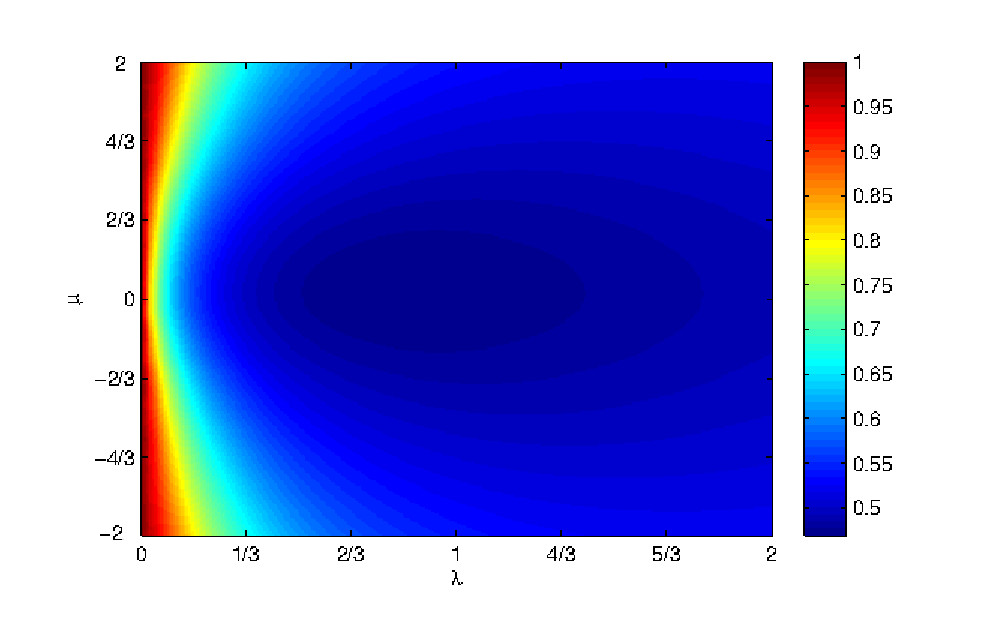
\epsfig{file=L01-L010-distance-e03-a03_mark2.eps, height=2.5in}
		\caption{Ukázka hodnot Rényiho pseudovzdálenosti s parametrem $\alpha = 0.3$ Laplaceově modelu. Data jsou generována jako konvexní směs Laplaceových distribucí $0.7\mathrm{L}(0,1) + 0.3 \mathrm{L}(0,10)$.}
		\label{fig-distanceL}
	\end{center}
\end{figure}

\begin{figure}[htb!]
	\begin{center}
		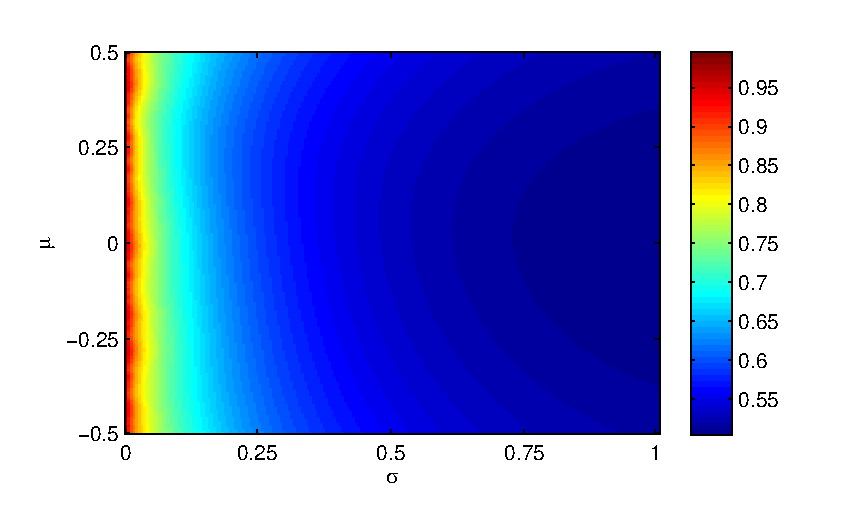
\epsfig{file=C01-err10x0.2-a05-dist.eps, height=2.5in}
		\caption{Detailnější pohled na hodnoty Rényiho pseudovzdálenosti s parametrem $\alpha = 0.5$. Data jsou z Cauchyho modelu s řádovou chybou $0.8\mathrm{C}(0,1) + 0.2 \mathrm{C}_{10}(0,1)$.}
		\label{fig-distanceC}
	\end{center}
\end{figure}

Sice jde jen o příklady, ale i pro jiná data vycházejí velmi podobné vizualizace. Obrázek \ref{fig-distanceC} je v poněkud větším detailu, takže je o něco lépe vidět, že ani ve větším přiblížení nemá funkce nějaké nepříjemné lokální extrémy. 

Dá se tedy říct, že minimalizovaná funkce je poměrně hladká a nejen, že není potřeba procházet celý stavový prostor pomocí metody sítí, ale dá se dokonce použít jednoduše modifikovaný "hill climber," který není zpomalovaný ani náhodným se vracením, které je tak důležité pro simulovaného žíhání. Pokud chceme dosáhnout dobré přesnosti, je potřeba, aby algoritmus procházel stavový prostor v malých krocích. To však není potřeba v průběhu celého běhu algoritmu, ale jen na jeho konci, proto jsme mohli začít s poněkud větším krokem a ten pak v dalších iteracích algoritmu zmenšovat. Náš minimalizační algoritmus tedy vypadá následovně: 
\vspace{11 pt} \\
\textbf{Minimalizační algoritmus "hill climber"}

\begin{enumerate}
	\item Zvolíme dvourozměrný interval $[a_1,a_2]\times [b_1,b_2]$, ve kterém budeme hledat minimum funkce $f$.
	\item Zvolíme počáteční krok metody $\varepsilon$ a požadovanou přesnost vyjádříme pomocí $\varepsilon_{\min}$
	\item Vyhodnotíme funkci v inicializačním bodě $x = (a,b),$ kde $a \in [a_1,a_2],\; b \in [b_1,b_2]$	
	\item Najdeme 8 bodů $\lbrace x_1,\ldots,x_8 \rbrace$ na rozích a uprostřed stran čtverce s délkou strany $2\varepsilon$ v jehož středu je bod $x$.	
	\item Pokud jsou body v námi prohledávané oblasti, najdeme $x_{\min} = \arg\min \lbrace f(x),f(x_1),\ldots,f(x_8)\rbrace$
		\begin{enumerate}
			\item Pokud je minima dosaženo v bodu $x_i \in \lbrace x_1,\ldots,x_8 \rbrace$, položíme $x := x_i$.
			\item Pokud je v bodě $x$ stále funkční hodnota nejmenší položíme $\varepsilon:= \frac{\varepsilon}{2}$.
		\end{enumerate}		
	\item Pokud platí $\varepsilon > \varepsilon_{\min}$, pokračujeme bodem 4. V opačném případě již máme bod $x$, v kterém je funkce $f$ minimální v požadované přesnosti.
\end{enumerate}

My jsme navíc měli situaci zjednodušenou tím, že jsme věděli, v jakém přibližně bodě bude funkce minimální, takže jsme i počáteční iteraci mohli umístit do blízkosti tohoto bodu. Pokud tedy bude někdy metoda používána aniž by uživatel kontroloval tvar minimalizované funkce na konkrétních datech, měl by se implementovat algoritmus, který si lépe poradí s lokálními extrémy, například již zmíněný algoritmus simulovaného žíhání.

Radim Demut v \cite{Demut2010} popisuje použití metody na Newcombových datech o měření světla, kde vzniklo několik lokálních extrémů.

\begin{figure}[htb!]
	\begin{center}
		\epsfig{file=E01-E101-e04-a05-dist.eps, height=2.5in}
		\caption{Rényiho pseudovzdálenost s parametrem $\alpha = 0.5$. Data jsou generovaná jako konvexní směs exponenciálních rozdělení $0.6\mathrm{E}(0,1) + 0.4\mathrm{E}(10,1)$.}
		\label{fig-distanceE}
	\end{center}
\end{figure}

Trochu jiný charakter má obrázek \ref{fig-distanceE}. Opět jde o vizualizaci Rényiho vzdálenosti na datech, nyní však v exponenciálním modelu. V horní části obrázku okolo správné polohy $\mu = 0$  hodnota pseudovzdálenosti roste směrem k zápornému $\hat{\mu}$ mnohem rychleji, protože většina dat (60\%) se nachází nad touto hranicí v oblasti $x<\mu$, tedy v horní čtvrtině obrázku. Podle \eqref{renyi-formula-exponential} přispívají k maximalizaci mnohem větší měrou, protože je výraz v exponenciální funkci v těchto případech kladný. Lokální minimum okolo bodu (10,1) je pak způsobeno 40\% dat, která měla rozdělení E(10,1).

\section{Výsledky experimentů}

V této části okomentujeme tabelované výsledky různých Rényiho odhadů. Níže se setkáme s následujícími statistikami:

\begin{align*}
	m(\gamma) = \frac{1}{K}\sum_{i=1}^K \widehat{\gamma}_{i},& \qquad s(\gamma) = \sqrt{\frac{1}{K}\sum_{i=1}^K (\widehat{\gamma}_{i}-\overline{\gamma})^2},\\
\end{align*}
kde $\gamma $ je kterýkoliv z odhadovaných parametrů. Ještě jsme pro porovnávání odhadů zavedli relativní eficienci 
\begin{equation}
	eref(\gamma) = \sqrt{\dfrac{\frac{1}{K}\sum_{i=1}^K (\widehat{\gamma}_{\mathrm{0} ,i} - \gamma_{\mathrm{real}})^2}{\frac{1}{i}\sum_{k=1}^K (\widehat{\gamma}_{\alpha,i} - \gamma_{\mathrm{real}})^2}},
\end{equation}
kde $\gamma_\mathrm{real}$ je hodnota parametru znečišťovaného rozdělení, $\gamma_{0,i}$ je použitý některý ze standardních odhadů daného parametru pro konkrétní rozdělení, $K$ je počet opakování odhadu. Standardní odhad $\gamma_{0,i}$ jsme volili maximálně věrohodný, pokud to šlo. Pro Normální a Laplaceovo jsme použili maximálně věrohodné odhady, stejně tak pro odhad měřítka $\lambda$ exponenciálního a Weibullova rozdělení. Vzhledem k definici exponenciálního rozdělení vzhledem k jeho parametru polohy $\mu$, tedy tomu, že pro všechna $x$ platí $x > \mu$, vzali jsme jako odhad $\mu$ minimální $x$ přítomné v datovém souboru.
Pro Cauchyovo rozdělení jsme použili odhady
\begin{equation}
	\widehat{\mu}  = \frac{X_{1-p} + X_{p}}{2}, \; p = 0.5565 \qquad \widehat{\sigma}  = \frac{X_{0.75} - X_{0.25}}{2}.
\end{equation}



\begin{figure}[htb]
	\begin{center}
		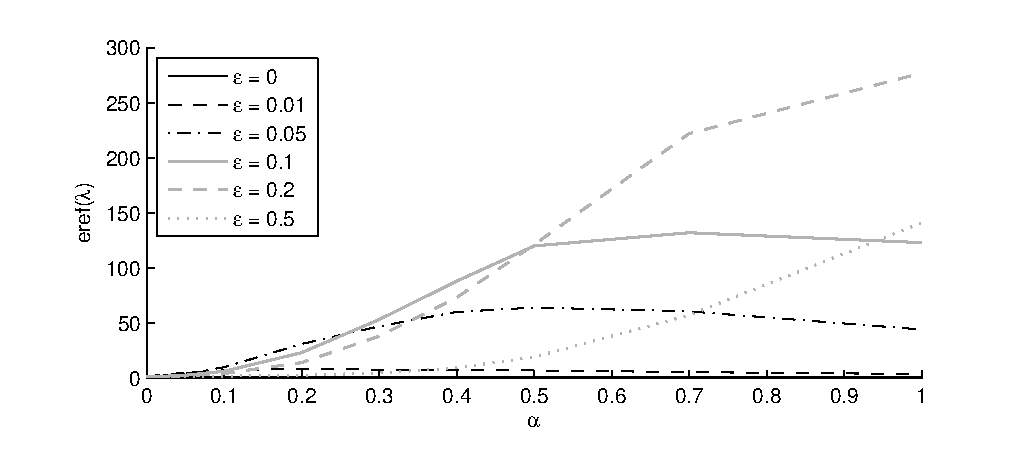
\epsfig{file=Eref-Exp-lambda.eps, height=2.in}
		\caption{Empirická relativní eficience eref($\hat{\lambda}$) minimálního $\mathfrak{R}_\alpha$-odhadu parametru $\lambda$ exponenciálního rozdělení v konvexní směsi 
		$(1-\varepsilon)E(0,1) + \varepsilon E(0,10)$ pro různá znečištění $\varepsilon$.}
		\label{fig-eref-Exp-lambda}
	\end{center}
\end{figure}

\begin{figure}[htb]
	\begin{center}
		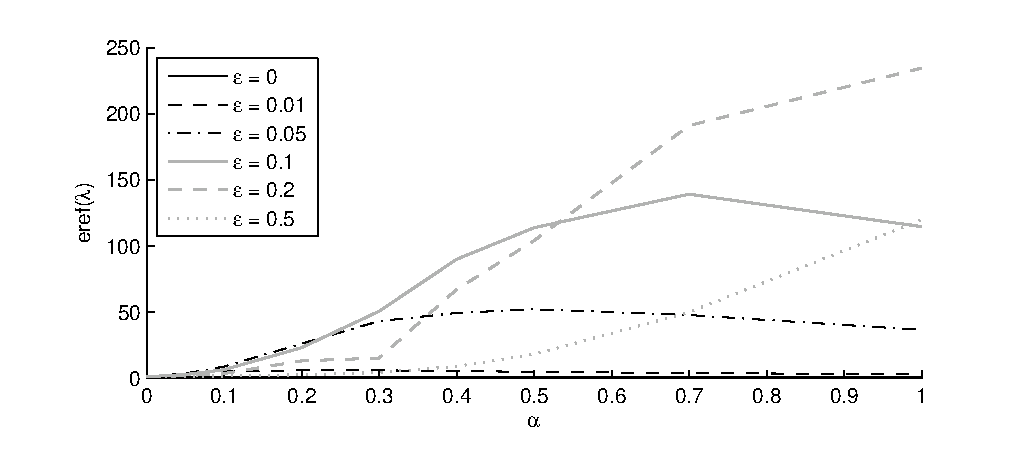
\epsfig{file=Eref-Laplace-lambda.eps, height=2.in}
		\caption{Empirická relativní eficience eref($\hat{\lambda}$) minimálního $\mathfrak{R}_\alpha$-odhadu parametrů  $\mu,\lambda$ Laplaceova rozdělení na datovém souboru o velikosti $n = 500$ generovaném	jako konvexní směs	$(1-\varepsilon)L(0,1) + \varepsilon L(0,10)$ pro různá znečištění $\varepsilon$.}
		\label{fig-eref-Laplace-lambda}
	\end{center}
\end{figure}

\begin{figure}[htb]
	\begin{center}
		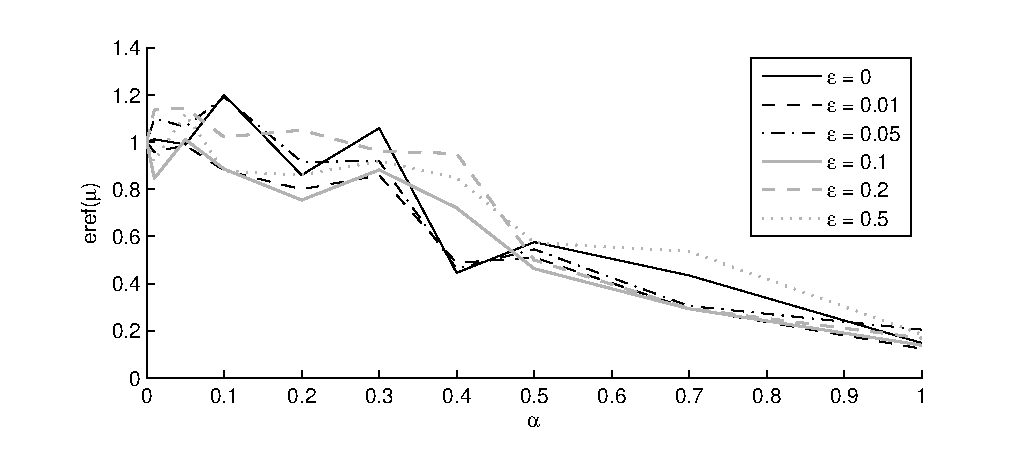
\epsfig{file=Eref-Exp-mu.eps, height=2.in}
		\caption{ TODO }
		\label{fig-eref-Exp-mu}
	\end{center}
\end{figure}

\begin{figure}[htb]
	\begin{center}
		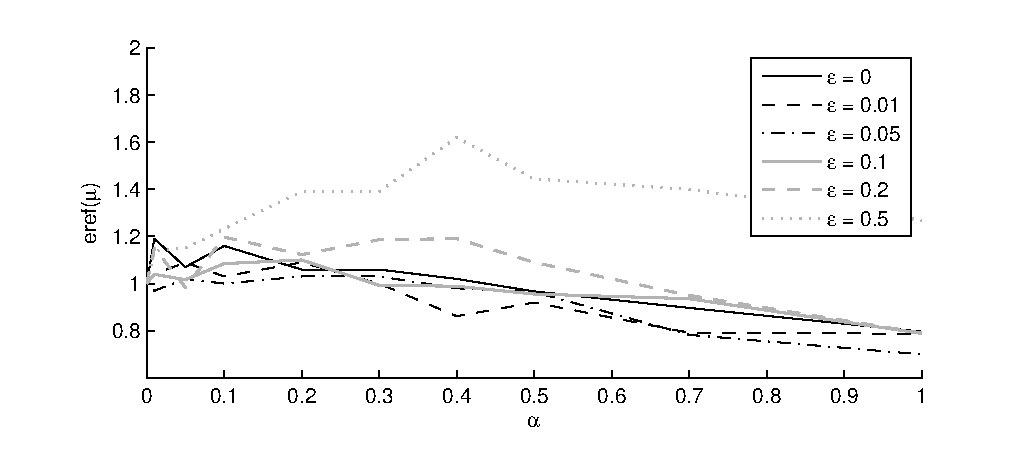
\epsfig{file=Eref-Laplace-mu.eps, height=2.in}
		\caption{ TODO }
		\label{fig-eref-Laplace-mu}
	\end{center}
\end{figure}

